%\documentclass[12pt]{article}
\documentclass[12pt]{extarticle}
\usepackage[utf8]{inputenc}
\usepackage[margin=0.5in]{geometry}
\usepackage{enumitem}
\usepackage{graphicx}
\usepackage{float}
\usepackage{romannum}
 
 % Title page
\title{VAST 2019 Weekly Report 2}
\author{Vivek Koodli Udupa}
\date{\today}

\begin{document}
\pagenumbering{arabic}
\maketitle

% INTRODUCTION
\begin{centering}
	\section{Introduction}
\end{centering}
This report will address the credibility of the damages reported by the citizens of St. Himark using the RUMBLE app. As addressed in Report 1, the number of damage reports coming in from different locations are unbalanced. Some locations have high number of reports where as some locations have very few entries. This report addresses ways to deal with this nonuniform distribution of data and analyzing the reliability of damages reported.  \\

% VISUALIZATION	
\begin{centering}
	\section{Visualization and Analysis}
\end{centering}

%Plot of Maps
\begin{figure}[H]
	\centering
	\begin{minipage}{0.5\textwidth}
		\centering
		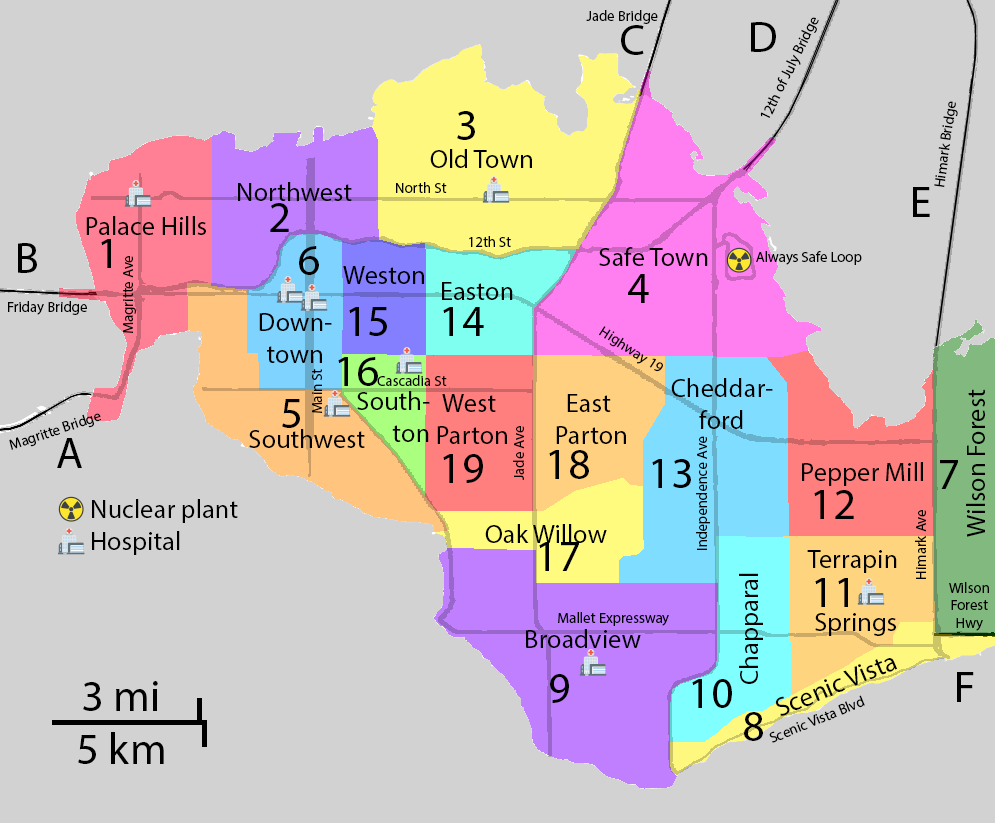
\includegraphics[width=\textwidth]{Images/map.png}
		\caption{St.Himark Neighborhood Map}
		\label{fig:map}
	\end{minipage}%
	\begin{minipage}{0.5\textwidth}
		\centering
		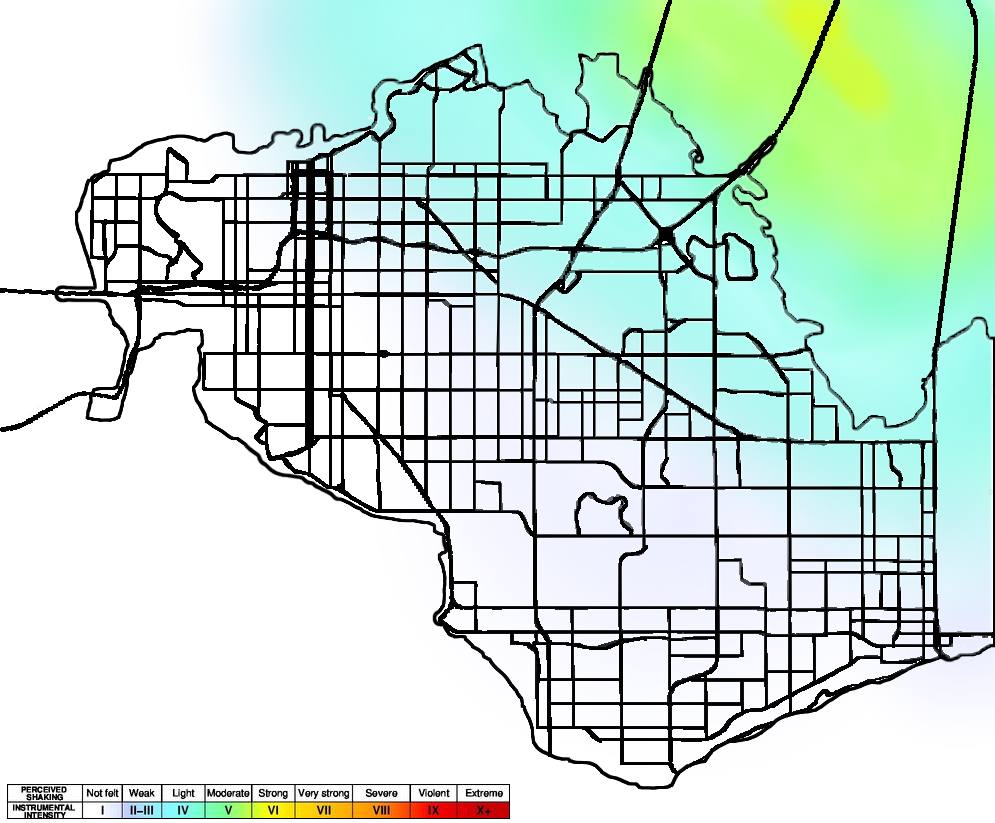
\includegraphics[width=\textwidth]{Images/shakemap.png}
		\caption{St.Himark Shake Map}
		\label{fig:shakemap}
	\end{minipage}
\end{figure} 

% Damage plot
\begin{figure}[H]
\centering
	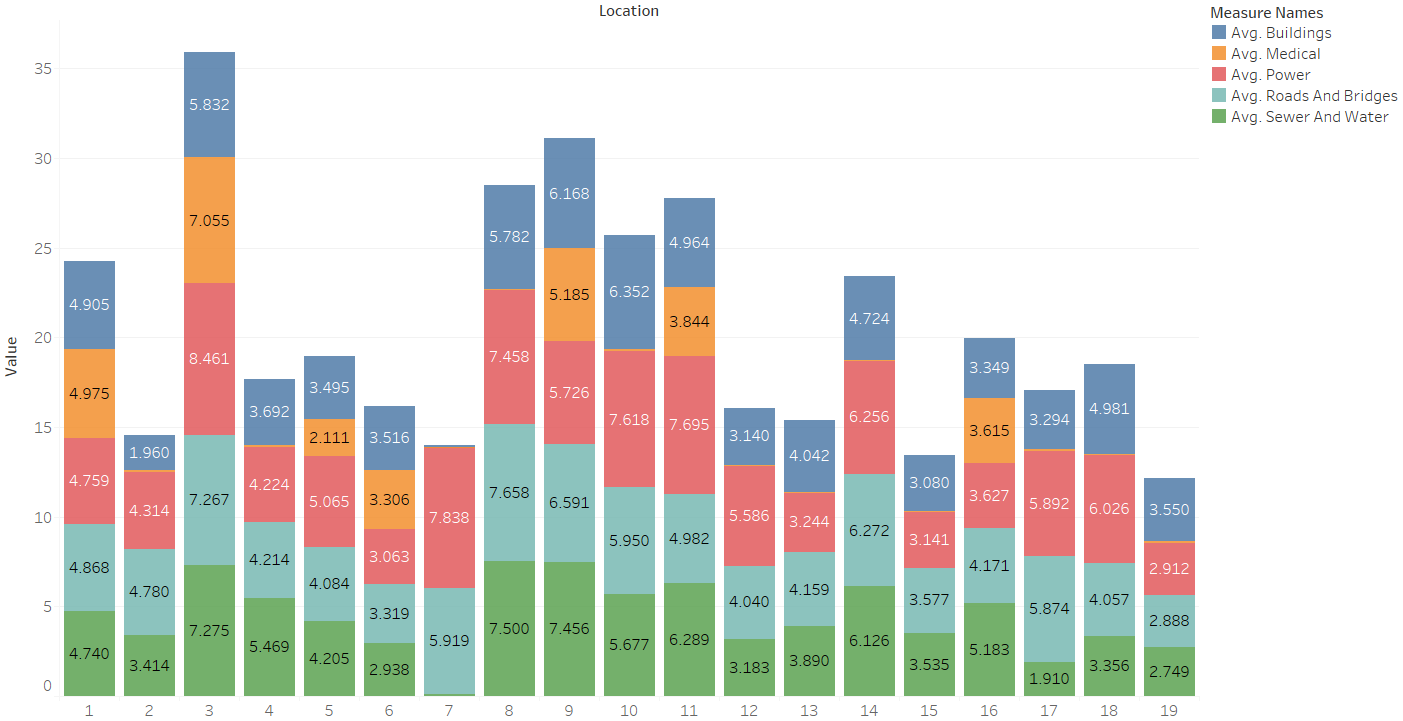
\includegraphics[width=\linewidth]{Images/AllDamage.png}
	\caption{Cumulative damage for different locations }
	\label{fig:alldamage}
\end{figure}

Figure \ref{fig:alldamage} shows the total damage sustained by different locations, which were observed and reported by the citizens of St. Himark. This figure raises suspicion. Locations 1, 8, 9, 10 and 11 shows relatively high damage even though they are not in the earthquake shake zone as shown in Figure \ref{fig:shakemap}. The high damage of Location 3 is acceptable as it resides directly in the shake zone. what could be the cause for the high damage reports in other locations? Are the data collected from RUMBLE reliable? \\

From the description of St. Himark [1] given in the documentation of VAST 2019 MiniChallenge 1, there were several ongoing road and water related repairs taking place before the earthquake disaster. These repairs caused road blocks and possibly inaccessibility to water for the citizens of St. Himark. Thus citizens might have reported damages even before the earthquake took place. \\
 


%Date Plot
\begin{figure}[H]
\centering
	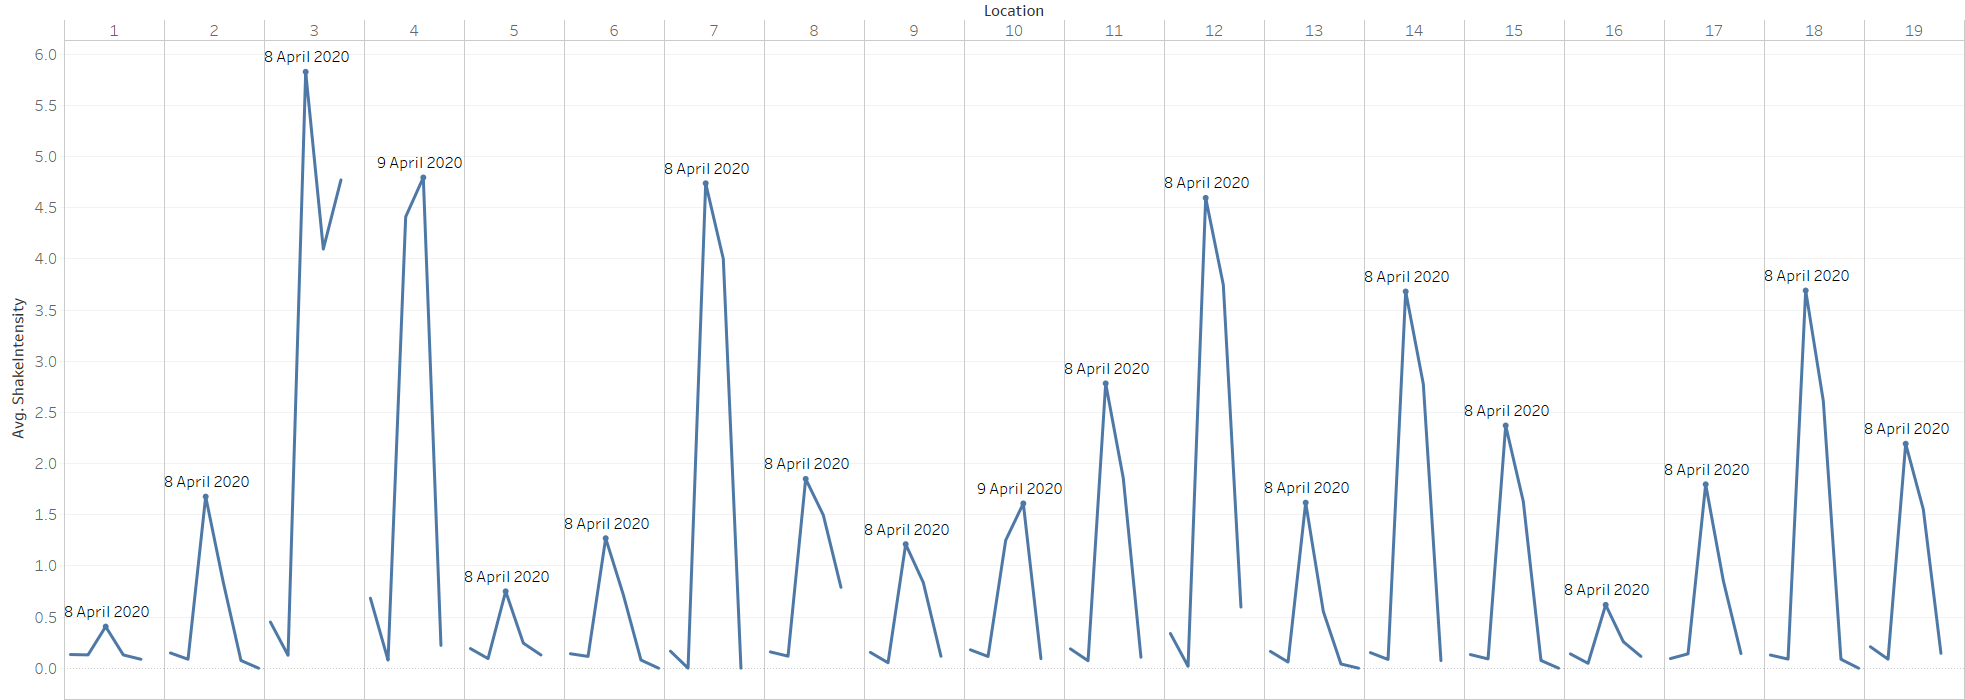
\includegraphics[width=\linewidth]{Images/Date.png}
	\caption{Date vs Shake intensity for all Locations }
	\label{fig:date}
\end{figure}

\begin{figure}[H]
\centering
	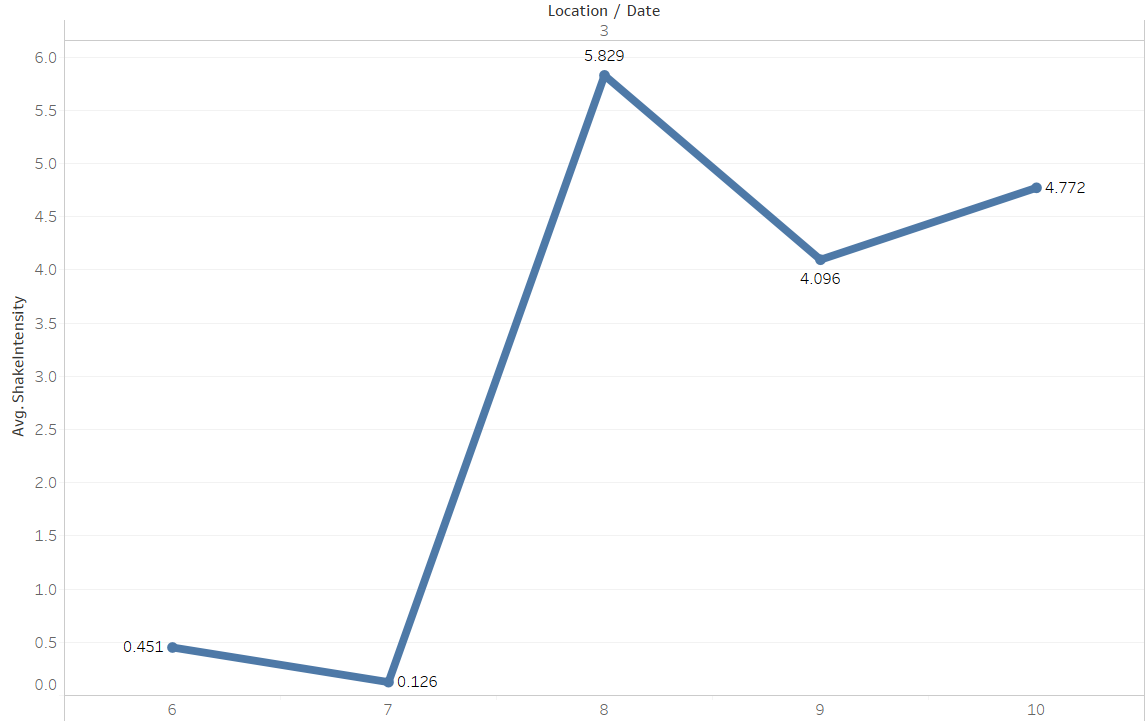
\includegraphics[width=0.5\linewidth]{Images/DateZoom.png}
	\caption{Date vs Shake intensity for Location 3 }
	\label{fig:dateZoom}
\end{figure}

%Time plot
\begin{figure}[H]
\centering
	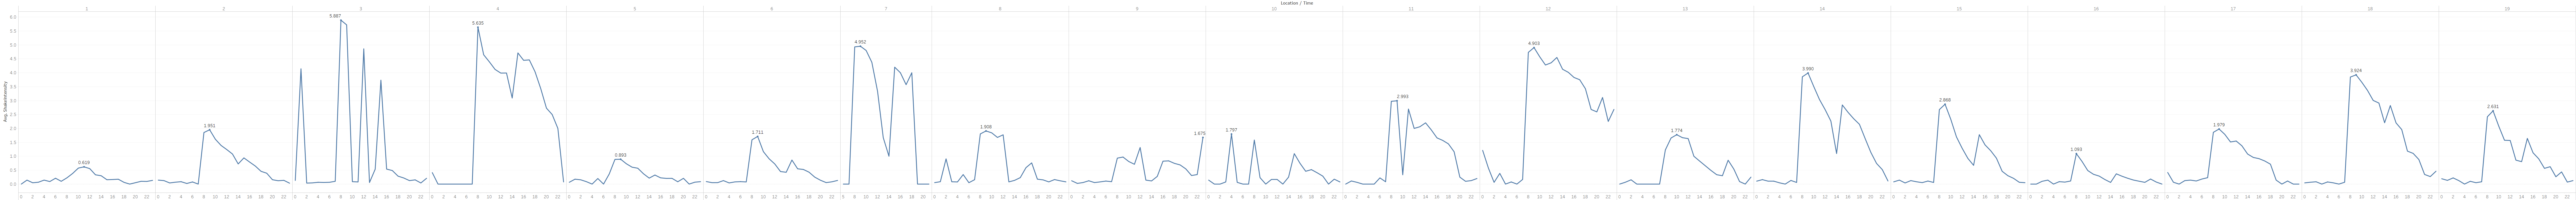
\includegraphics[width=\linewidth]{Images/time.png}
	\caption{Time of Earthquake}
	\label{fig:time}
\end{figure}

\begin{figure}[H]
\centering
	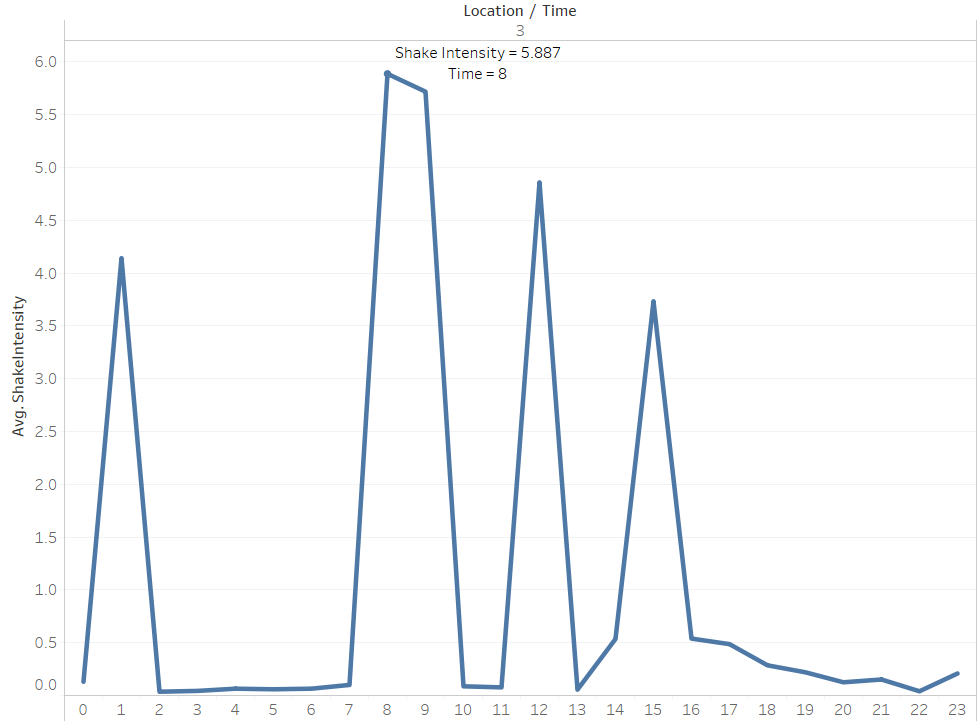
\includegraphics[width=0.5\linewidth]{Images/timeZoom.png}
	\caption{Time of Earthquake Zoomed into Location 3}
	\label{fig:timeZoom}
\end{figure}

% Mode Plot for Location 1
\begin{figure}[H]
\centering
	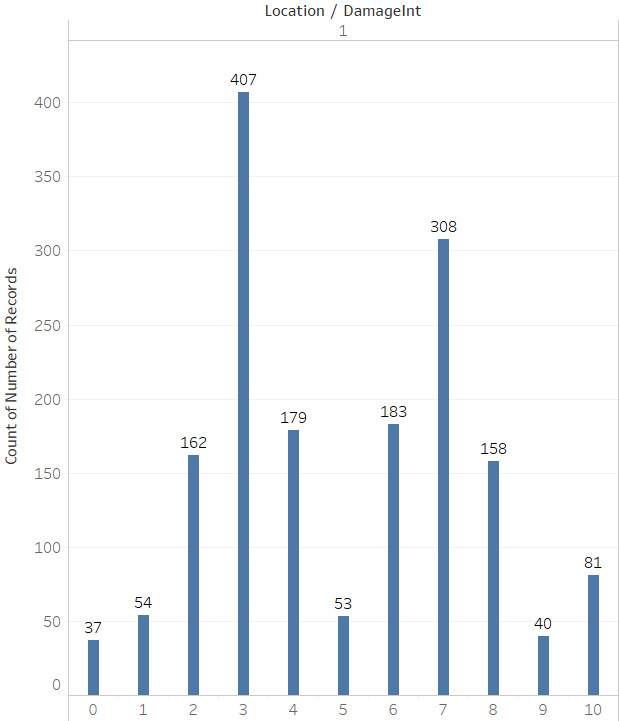
\includegraphics[width=0.5\linewidth]{Images/Loc1Mode.png}
	\caption{Number of Reports for different damage intensity at location 1 }
	\label{fig:mode}
\end{figure}

\begin{centering}
	\section{Conclusion}
\end{centering}

\begin{centering}
	\section{Reference}
\end{centering}
[1] VAST 2019 - St. Himark -  About our City.docx

\end{document}


